\documentclass[english,russian,a4paper,10pt]{article}
\usepackage[utf8]{inputenc}
\usepackage[T2A]{fontenc}
\usepackage{babel}
\usepackage{csquotes}

\usepackage{fullpage}
\usepackage{indentfirst}
\usepackage[font=small,labelfont=bf,labelsep=period]{caption}
\usepackage{graphicx}
\usepackage{wrapfig}
\usepackage{floatflt}

\usepackage{amssymb, amsmath}

\usepackage[
	pdfauthor={Oleg Rogozin},
	pdftitle={Heat and mass transfer simulation of compressible gas in continuum limit},
	colorlinks,pdftex, unicode]{hyperref}

\newcommand{\Kn}{\mathrm{Kn}}
\newcommand{\dd}{\:\mathrm{d}}
\newcommand{\pder}[2][]{\frac{\partial#1}{\partial#2}}
\newcommand{\pderder}[2][]{\frac{\partial^2 #1}{\partial #2^2}}

\usepackage[
	backend=biber,
	style=numeric,
	natbib=true,
	maxbibnames=99, minbibnames=99,
	language=american,
	babel=other,
	sorting=none,
	url=false,
	eprint=false,
	pagetracker,
	firstinits]{biblatex}
\bibliography{asymptoticSBFoam}

\title{
	\hbox{\normalsize УДК 532.5.013.3, 519.688}\hbox{}
	Моделирование теплопередачи и конвекции сжимаемого газа в континуальном пределе
}
\author{Рогозин Олег}
\date{}

\begin{document}

\maketitle
\begin{abstract}
	Для стационарного идеального газа перенос тепла в континуальном пределе (число Кнудсена стремится к нулю)
	не описывается классическим уравнением теплопроводности. Для описания процесса теплопередачи необходимо
	использовать более сложные уравнения, получаемые асимптотически из кинетической теории.
	На базе вычислительной платформы OpenFOAM\textregistered{} был разработан специальный солвер
	для решения подобных задач в произвольной геометрии.
	Выполнены характерные расчёты, указывающие на несправедливость классического уравнения теплопроводности
	для покоящегося газа.

	\hbox{}\noindent \textbf{Ключевые слова:}
	численное моделирование, уравнение Больцмана, уравнения Навье"--~Стокса, тепловое скольжение, термострессовая конвекция.
\end{abstract}


\section{Введение}

Для описания газа с бесконечно малой длиной свободного пробега (в континуальном пределе)
широко используются уравнения Навье"--~Стокса.
Но в ряде задач их решение некорректно описывает поля температуры~\cite{Kogan1976,Bobylev1996}.

Рассмотрим газ, окружающий покоящиеся тела в ограниченном пространстве
(для неограниченной области подразумевается, что на бесконечности скорость газа равна нулю, а давление постоянно).
В таком случае стационарное состояние с нулевой скоростью и постоянным давлением является
очевидным решением уравнений Навье"--~Стокса, а температурное поле описывается
классическим уравнением теплопроводности.
Тщательный асимптотический анализ кинетического уравнения Больцмана, однако, приводит
к более сложной системе уравнений для вычисления температурного распределения~\cite{Bobylev1996}.

В настоящей работе приведены соответствующие уравнения асимптотической теории взамен
уравнений классической гидродинамики и рассмотрены соответствующие двумерные задачи для сравнения
получаемых решений. Для этой цели был разработан специальный солвер в рамках существующей
проблемно-моделирующей среды~\cite{Rogozin2011, Martynov2011}.

\section{Основные уравнения}

Для описания жидкости и газа в общем виде используются уравнения сохранения массы, импульса и энергии:
\begin{gather}
	\pder[\rho]{t} + \pder{x_i}(\rho v_i) = 0, \label{eq:mass}\\
	\pder{t}(\rho v_i) + \pder{x_j}(\rho v_i v_j + p_{ij}) = \rho F_i, \label{eq:momentum}\\
	\pder{t}\left[\rho\left(e+\frac{v_i^2}2\right)\right] +
		\pder{x_j}\left[\rho v_j\left(e+\frac{v_i^2}2\right)+v_i p_{ij}+q_j\right] = \rho v_j F_j. \label{eq:energy}
\end{gather}
Макроскопические параметры: \(\rho\) "--- плотность, \(v_i\) "--- скорость, \(p_{ij}\) "--- тензор напряжений,
\(e\) "--- удельная внутренняя энергия, \(q_i\) "--- тепловой поток. \(F_i\) "--- внешняя сила.
Для идеального одноатомного газа внутренняя энергия~\(e\) зависит только от температуры~\(T\):
\[ e = \frac32RT,\]
где \(R=k_B/m\) "--- удельная газовая постоянная. Давление выражается через уравнение состояния:
\[ p = \rho RT. \]

Уравнения сохранения замыкаются до уравнений Навье"--~Стокса законами Ньютона и Фурье
для тензора напряжений \(p_{ij}\) и потока тепла \(q_i\) соответственно:
\begin{gather}
	p_{ij} = p\delta_{ij} - \mu\left(\pder[v_i]{x_j}+\pder[v_j]{x_i}-\frac23\pder[v_k]{x_k}\delta_{ij}\right) -
		\mu_B\pder[v_k]{x_k}\delta_{ij}, \label{eq:stress_tensor}\\
	q_i = -\lambda\pder[T]{x_i}. \label{eq:heat_flow}
\end{gather}
Здесь \(\mu\) "--- вязкость, \(\mu_B\) "--- вторая вязкость, \(\lambda\) "--- теплопроводность.

Число Кнудсена \(\Kn\) определяет отношение длины свободного пробега
\begin{equation}\label{eq:ell}
	\ell = \frac{m}{\sqrt2\pi d_m^2 \rho}.
\end{equation}
к характерному размеру задачи \(L\):
\begin{equation}\label{eq:Knudsen}
	\Kn = \frac{\ell}L.
\end{equation}
Далее будем использовать модифицированное число Кнудсена:
\begin{equation}
	k = \frac{\sqrt\pi}2\Kn.
\end{equation}

Для модели твёрдых сфер радиус действия межмолекулярного потенциала взаимодействия \(d_m\)
совпадает с диаметром.

Для идеального газа вязкость \(\mu\) и теплопроводность \(\lambda\)
пропорциональны длине свободного пробега \(\ell\), а значит и числу Кнудсена:
\begin{equation}
	\mu = O(k), \quad \lambda = O(k).
\end{equation}
При \(k\to0\) получается система уравнений Эйлера:
\begin{equation}
	p_{ij} = p\delta_{ij}, \quad q_i = 0.
\end{equation}

Однако из системы уравнений Эйлера нельзя определить поле температуры.
Классическое уравнение теплопроводности получается из~\eqref{eq:energy} и~\eqref{eq:heat_flow}
в предположении отсутствия потоков газа \(v_i = 0\):
\begin{equation}\label{eq:heat_equation}
	\pder{x_i}\left(\sqrt{T}\pder[T]{x_i}\right) = 0.
\end{equation}
Здесь учтено, что теплопроводность идеального газа пропорциональна \(\sqrt{T}\).

При малых значениях \(k\) в уравнениях Навье"--~Стокса возникает слабый конвекционный поток \(v=O(k)\),
уравновешивающий член теплопроводности в~\eqref{eq:energy}.
Несмотря на своё исчезновение при \(k\to0\), он конечным образом влияет на температурное поле.
Описать данное влияние можно только из кинетической теории, используя асимптотический анализ 
уравнения Больцмана при малых числах Кнудсена.

\section{Асимптотический анализ уравнения Больцмана}
Подробный математический вывод приведённых ниже результатов можно найти в~\cite{Sone2002}.

Для анализа используется классическое разложение Гильберта~\cite{Hilbert1912}
функции распределения \(f\) и макропараметров \(h\):
\[ f = f_0 + f_1k + f_2k^2 + \cdots, \]
\[ h = h_0 + h_1k + h_2k^2 + \cdots \]
при дополнительном условии
\begin{equation}\label{eq:Mach_constraint}
	\int\xi_if\dd\xi = O(k),
\end{equation}
означающем, что число Маха такого же порядка малости, что и число Кнудсена.

Конечным результатом является следующая стационарная система уравнений для \(T_0\), \(u_{i1} = p_0v_{i1}\), \(p_2\):
\begin{align}
	\pder{x_i}\left(\frac{u_{i1}}{T_0}\right) &= 0, \label{eq:asymptotic1} \\
	\pder{x_j}\left(\frac{u_{i1}u_{j1}}{T_0}\right)
		&-\frac{\gamma_1}2\pder{x_j}\left[\sqrt{T_0}\left(
			\pder[u_{i1}]{x_j}+\pder[u_{j1}]{x_i}-\frac23\pder[u_{k1}]{x_k}\delta_{ij}\right
		)\right] \notag\\
		&- \frac{\gamma_7}{T_0}\pder[T_0]{x_i}\pder[T_0]{x_j}\left(\frac{u_{j1}}{\gamma_2\sqrt{T_0}} - \frac{1}4\pder[T_0]{x_j}\right) \notag\\
		&= -\frac1{2p_0}\pder[p_2^\dag]{x_i}, \label{eq:asymptotic2} \\
	\pder[u_{i1}]{x_i} &= \frac{\gamma_2}2\pder{x_i}\left(\sqrt{T_0}\pder[T_0]{x_i}\right). \label{eq:asymptotic3}
\end{align}
Давления \(p_0\), \(p_1\) являются константами,
\[ 
	p_2^\dag = p_2 + 
		\frac{2\gamma_3}{3p_0}\pder{x_k}\left(T_0\pder[T_0]{x_k}\right) -
		\frac{\gamma_7}{6p_0}\left(\pder[T_0]{x_k}\right)^2,
\]
Система \eqref{eq:asymptotic1}--\eqref{eq:asymptotic3} носит гидродинамический характер
и сравнима с уравнениями Навье"--~Стокса для сжимаемого газа (\(\rho_0 = p_0/T_0\)).
Формальная разница в дополнительных членах термических напряжений.
Кроме того, \(p_2^\dag\) не входит в уравнение состояния, поэтому определяется с точностью до константы.
Член \(\partial{p_2^\dag}/\partial{x_i}\) включён в систему,
как давление в уравнениях Навье"--~Стокса для несжимаемого газа,
что определяет соответствующие методы решения приведённой системы.

Для модели твёрдых сфер безразмерные коэффициенты переноса равны
\begin{alignat*}{2}
	\gamma_1 &= 1.270042427, &\quad \gamma_2 &= 1.922284066, \\
	\gamma_3 &= 1.947906335, &\quad \gamma_7 &= 1.758705.
\end{alignat*}

Первые два коэффициента соответствуют вязкости и теплопроводности:
\[ \mu = \frac{\sqrt\pi}2\gamma_1, \quad \lambda = \frac{5\sqrt\pi}2\gamma_2. \]

Граничные условия на границе с диффузным отражением имеют вид:
\begin{gather}
	T_0 = T_w, \label{eq:bound:T} \\
	\left\{
	\begin{aligned}
		& \frac{(u_{j1}-u_{wj1})}{\sqrt{T_w}}(\delta_{ij}-n_in_j) = 
			-K_1\pder[T_w]{x_j}(\delta_{ij}-n_in_j), \\
		& u_{j1}n_j = 0.
	\end{aligned}
	\right. \label{eq:bound:v}
\end{gather}
Здесь \(n_i\) "--- нормаль к поверхности, \(u_{wj1}\), \(T_w\) "--- скорость и температура границы.
\(K_1\) "--- безразмерный коэффициент температурного скачка. Для модели твёрдых сфер 
\[ K_1 = -0.6463. \]

\begin{wrapfigure}{r}{6.5cm}
	\vspace{-10pt}
	\includegraphics{transport/Y1}
	\vspace{-20pt}
	\caption{Функция \(Y_1(\eta)\) кнудсеновского слоя для модели твёрдых сфер}\label{fig:Y1}
	\vspace{5pt}
\end{wrapfigure}

Полученное решение в общем случае не может точно удовлетворить кинетическому граничному условию
ввиду резкого изменения функции распределения у границы вдоль нормали к ней.
Поэтому необходимо вводить так называемую коррекцию кнудсеновского слоя:
\begin{equation}
	f = f_{FD} + f_K.
\end{equation}
Гидродинамическая часть \(f_{FD}\) представляет собой полученное ранее решение,
а \(f_K\) убывает экспоненциально от расстояния до границы \(\eta\):
\begin{equation}
	f_K = O\left(e^{-\eta}\right), \quad \eta = \frac{x_in_i}k.
\end{equation}

Ввиду малости числа Маха (\ref{eq:Mach_constraint}) \(f_K\) разлагается в ряд, начиная с первого порядка малости:
\[ f_K = f_{K1}k + f_{K2}k^2 + \cdots \]
Учёт кнудсеновского слоя вводит поправку для \(u_{i1}\) для модели твёрдых сфер:
\begin{equation}
	\left\{
	\begin{aligned}
		& \frac{u_{jK1}}{\sqrt{T_w}}(\delta_{ij}-n_in_j) = 
			-\frac12\pder[T_w]{x_j} Y_1\left(\frac\eta{T_w}\right) (\delta_{ij}-n_in_j), \\
		& u_{jK1}n_j = 0.
	\end{aligned}
	\right. \label{eq:bound:v_K}
\end{equation}
Функция \(Y_1(\eta)\) табулирована, например, в~\cite{Sone2002, Sone2007} и изображена на рис.~\ref{fig:Y1}.

Видно, что при \(\Kn\to0\) газ в общем случае не описывается уравнением теплопроводности~\eqref{eq:heat_equation}.
Уравнение~\eqref{eq:asymptotic3} сходится к нему только в частном случае при \(u_{i1} = 0\).
Можно выделить три причины, по которым это условие не выполняется:
\begin{enumerate}
	\item Граница движется с инфинитезимальной скоростью: \(u_{wi} = u_{w1i}k\).
	\item Температура границы неравномерна (тепловое скольжение).
	\item Изотермические поверхности не параллельны (термострессовая конвекция)~\cite{Kogan1976}:
		\begin{equation}\label{eq:equilibrium}
			e_{ijk}\pder[T_0]{x_j}\pder{x_k}\left(\pder[T_0]{x_l}\right)^2 = 0.
		\end{equation}
\end{enumerate}

Первые два случая напрямую определяются граничными условиями, третий же только косвенно зависит
от них.

\section{Численное моделирование}

\begin{wrapfigure}{r}{6cm}
	\vspace{-20pt}
	\centering
	\includegraphics{tikz/bobylev}
	\vspace{-20pt}
	\caption{Геометрия задачи}\label{fig:geometry}
	\vspace{-5pt}
\end{wrapfigure}

Для решения системы уравнений~\eqref{eq:asymptotic1}--\eqref{eq:asymptotic3} был разработан
специальный солвер на основе готовой вычислительной платформы OpenFOAM\textregistered{}~\cite{Tabor1998},
использующей метод конечных объёмов.
Уравнение непрерывности~\eqref{eq:asymptotic1} вместе с уравнением импульса~\eqref{eq:asymptotic2}
решаются с помощью классического неявного консервативного алгоритма SIMPLE~\cite{Caretto1972}.
В качестве генератора неструктурированных сеток используется пакет GMSH~\cite{Geuzaine2009}.

Все транспортные коэффициенты взяты для модели твёрдых сфер.
От твёрдых поверхностей предполагается полное диффузное отражение.

Использовались неравномерные пространственные сетки, сгущающиеся в области б\'{о}льших градиентов макропараметров.
Невязка конечного решения во всех задачах не превышает \(10^{-6}\).

\subsection{Газ между двумя параллельными пластинами}

Рассмотрим плоскую периодическую геометрию, схематически изображённую на рис.~\ref{fig:geometry}.
Газ помещён между двумя бесконечными параллельными пластинами.
Температура на них распределена по синусоидальному закону:
\begin{equation}
	T_w = 1-\alpha\cos(2\pi x).
\end{equation}
Нижняя пластина относительно верхней движется со скоростью
\begin{equation}
	u_{wi} = (\beta \Kn,0,0).
\end{equation}

Рассмотрим частный случай:
\[\alpha=1/2, \quad \beta = 1. \]

В силу симметрии задачи расчётная область будет представлять собой прямоугольник
(на рис.~\ref{fig:geometry} выделен серым цветом).

\begin{figure}[ht]
	\centering
	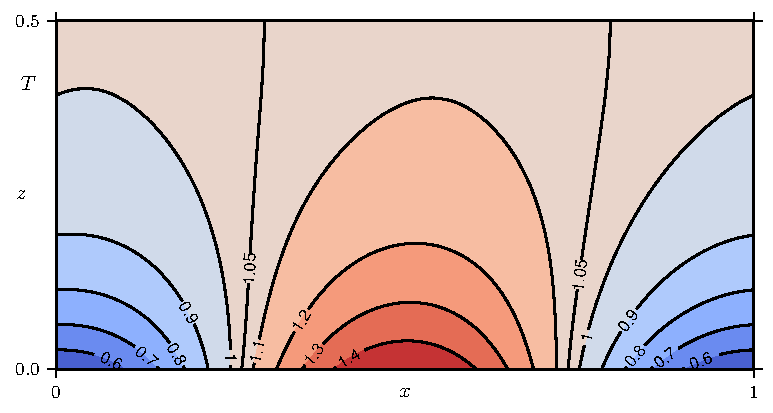
\includegraphics{moving_wall/T_asym}
	\caption{Поле температуры \(T\), полученное из асимптотической теории}
	\label{fig:moving:T_asym}
\end{figure}

\begin{figure}[ht]
	\centering
	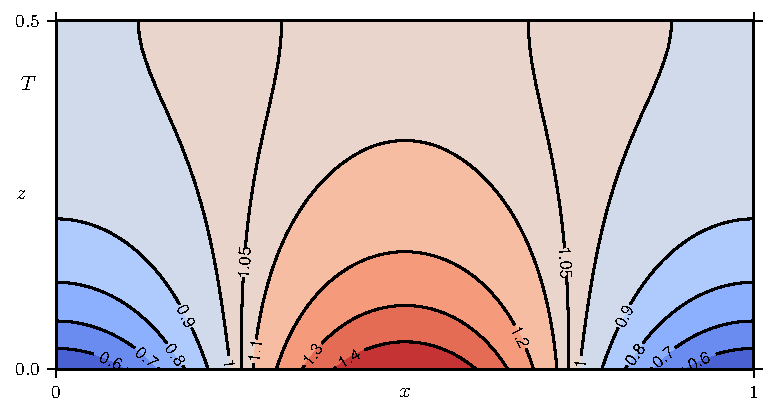
\includegraphics{moving_wall/T_heat}
	\caption{Поле температуры \(T\), полученное из уравнения теплопроводности}
	\label{fig:moving:T_heat}
\end{figure}

\begin{figure}[ht]
	\centering
	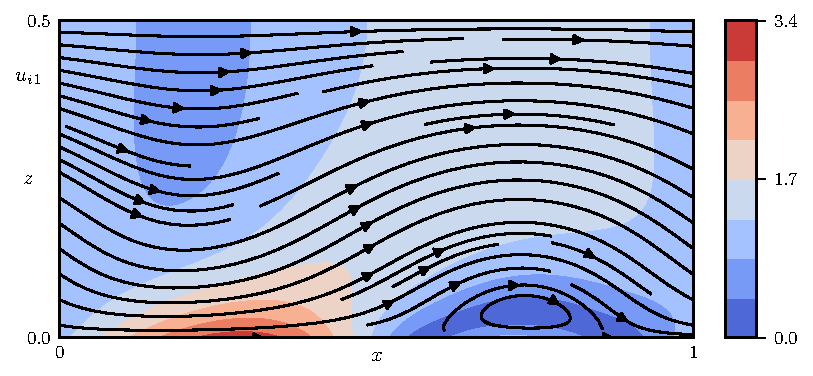
\includegraphics{moving_wall/U_0}
	\caption{Поле скоростей \(u_{i1}\) при \(\Kn=0\)}\label{fig:moving:fluid}
\end{figure}

\begin{figure}[ht]
	\centering
	\includegraphics{moving_wall/U_001}
	\caption{Поле скоростей \(u_{i1}\) при \(\Kn=0.01\) }\label{fig:moving:kn001}
\end{figure}

Искомое распределение температуры в гидродинамическом пределе изображено
на рис.~\ref{fig:moving:T_asym} в сравнении с решением уравнения теплопроводности (рис.~\ref{fig:moving:T_heat}).
Видно, что классическое решение несколько отличается от точного кинетического при \(k\to0\).

Далее показано поле скоростей \(u_{i1}\) для предельного (рис.~\ref{fig:moving:fluid})
и конечного чисел Кнудсена (рис.~\ref{fig:moving:kn001}).
Последний рисунок получен с учётом корректировки кнудсеновского слоя~\eqref{eq:bound:v_K}.

Таким образом видно, что при малых числах Кнудсена возникает пристеночное движение газа
вдоль градиента температуры твёрдой поверхности, называемое \textit{тепловым скольжением}.
Это эффект первого порядка малости по \(k\).

В гидродинамическом пределе поле скоростей стремится к нулю:
\[ u_i = u_{i1}k + O(k^2) \to 0, \quad k\to0,\]
однако \(u_{i1}\) остаётся конечным и трансформирует поле температуры через~\eqref{eq:asymptotic3}.

Кроме того, важно отметить, что решение задачи очень чувствительно к взаимной скорости движения пластин.
Бесконечно малая \(u_w\) также конечным образом влияет на поле температур через \(u_{w1}\).

\subsection{Газ между двумя цилиндрами и сферами}

\begin{figure}[ht]
	\centering
	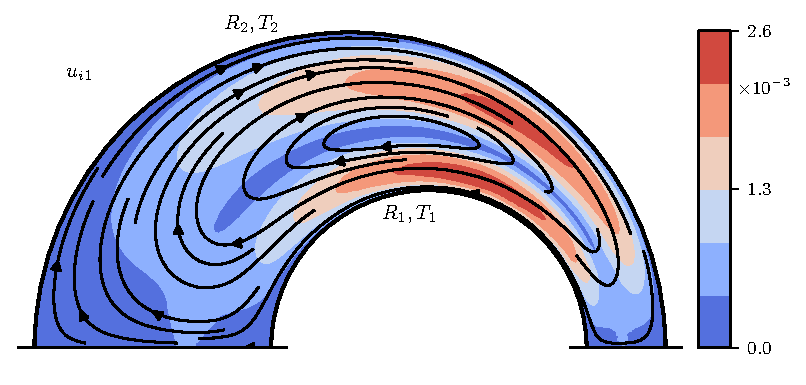
\includegraphics{noncoaxial/cylinders}
	\caption{Стационарное поле \(u_{i1}\) между двумя некоаксиальными цилиндрами}\label{fig:cylinders}
\end{figure}

\begin{figure}
	\centering
	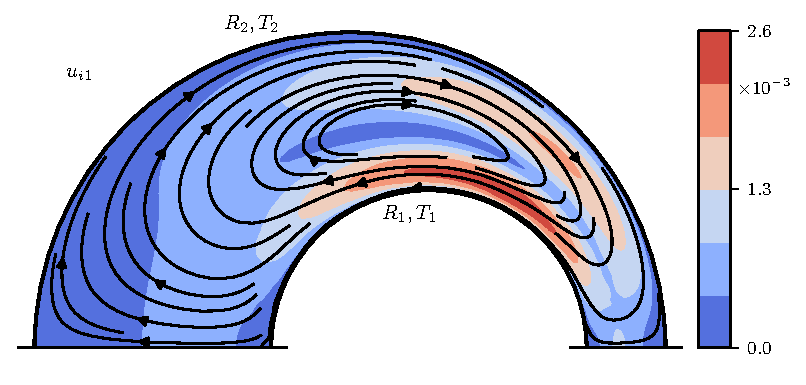
\includegraphics{noncoaxial/spheres}
	\caption{Стационарное поле \(u_{i1}\) между двумя неконцентрическими сферами}\label{fig:spheres}
\end{figure}

Теперь рассмотрим случай отсутствия градиента температур на покоящихся обтекаемых телах.
Как было указано ранее, даже при таких граничных условиях может возникать конвекционные потоки,
обусловленные непараллельностью изотермических поверхностей~\eqref{eq:equilibrium}.

Это явление было названо \textit{термострессовой конвекцией} и впервые описано в~\cite{Kogan1971}.
Важное особенностью является нелинейное происхождение этого эффекта в первом порядке малости по числу Кнудсена.
В линейной асимптотической теории термострессовая конвекция возникает лишь в следующем порядке малости \(O(k^2)\).

Особенность данного типа конвекции заключается в том, что она может протекать в условиях невесомости,
в то время как для возбуждения классической конвекции необходимо поле тяжести.

Рассмотрим два цилиндра радиусами \(R_1=1\) и \(R_2=r\)
с температурами \(T_1=1\) и \(T_2=\alpha\) соответственно.
Оси цилиндров параллельны, расстояние между ними равно \(d\).

На рис.~\ref{fig:cylinders} представлены результаты численного моделирования для частного случая:
\[ r = 2, \quad d = 1/2, \quad \alpha = 2.\]

Возникающее поле скоростей \(u_{i1}\) на несколько порядков ниже, чем в предыдущей задаче, поэтому практически не влияет на температурное распределение.

Вместо цилиндров можно смоделировать задачу с неконцентрическими сферами в такой же геометрической постановке,
тогда картина скоростей примет вид, как на рис.~\ref{fig:spheres}.

\subsection{Газ между двумя эллиптическими цилиндрами}

\begin{figure}
	\centering
	\includegraphics{elliptic/U}
	\caption{Стационарное поле \(u_{i1}\) между коаксиальными эллиптическими цилиндрами}
	\label{fig:elliptic}
\end{figure}

Последней рассмотрим задачу, в которой газ помещён между двумя коаксиальными эллиптическими цилиндрами,
так что главные оси эллипсов в поперечном сечении были перпендикулярны.
За единичное расстояние возьмём малую полуось внешнего цилиндра, большая тогда равна \(a_1\).
Внутренний эллипс имеет соответственно полуоси \(b_0\) и \(a_0\).
Температуры также равны \(T_1=1\), \(T_2=\alpha\).

Рассмотрим частный случай:
\[ a_1 = 1.5, \quad a_0 = 0.3, \quad b_0 = 0.7, \quad \alpha = 2.\]

Численное моделирование разреженного газа методом DSMC в описанной геометрии
для широкого диапазона чисел Кнудсена \(0.1\le\Kn\le5\) можно найти в~\cite{Sone1998}.

\begin{figure}[ht]
	\centering
	\begin{minipage}{.48\textwidth}
		\centering
		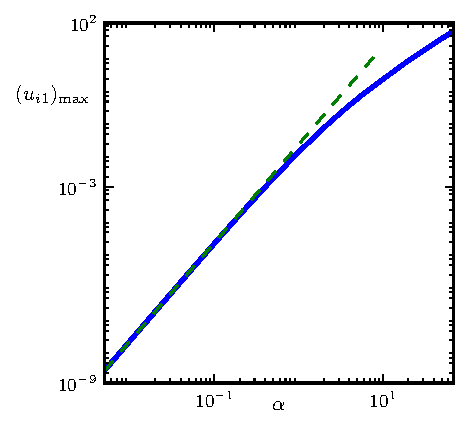
\includegraphics{elliptic/alpha}
		\captionof{figure}{Максимальное значение модуля \(u_{i1}\) в зависимости от отношения температур цилиндров \(\alpha\)}
		\label{fig:maxU}
	\end{minipage}
	\quad
	\begin{minipage}{.48\textwidth}
		\centering
		\includegraphics{elliptic/temper}
 		\vspace{-11pt}
		\captionof{figure}{Разность температурных полей \(\delta T\) вдоль оси \(x\) для \(\alpha=5\)}
		\label{fig:deltaT}
	\end{minipage}
\end{figure}

Время расчёта подобной задачи на современном персональном компьютере составляет несколько минут,
что позволяет оперативно выполнять параметрические исследования в том числе. Как пример,
на рис.~\ref{fig:maxU} показана зависимость максимального значения \(u_{i1}\) в зависимости от \(\alpha\).
Для малых \(\alpha\) справедлива кубическая зависимость:
\begin{equation}
	\mathrm{max}(u_{i1}) \propto \alpha^3.
\end{equation}

Наконец, на рис.~\ref{fig:deltaT} показана характерная разность между температурными полями,
полученными из асимптотической теории и уравнения теплопроводности
\[ \delta T = T_\mathrm{asym} - T_\mathrm{heat} \]
вдоль большей оси внешнего эллиптического цилиндра.

\section{Заключение}

В гидродинамическом пределе (\(\Kn\to0\)) распределение газа является максвелловским,
но макроскопические переменные в нём не удовлетворяют ни уравнениям Эйлера,
ни уравнениям Навье"--~Стокса. Они определяются системой уравнений,
содержащей члены более высокого порядка разреженности газа.

Разработанный солвер для корректной системы уравнений и соответствующих граничных условий
позволяет быстро и с высокой точностью решать поставленные задачи для произвольной геометрии.

В рассмотренных задачах были наглядно показаны температурные эффекты слабо разреженного газа:
тепловое скольжение и термострессовая конвекция.

\printbibliography

\end{document}


